\documentclass[11pt,a4paper]{scrreprt}
\usepackage{graphicx}
\usepackage[ngerman]{babel} 
\usepackage[T1]{fontenc}
\usepackage[utf8]{inputenc} 
\usepackage{setspace}
\usepackage{tabularx}
\usepackage{wrapfig}
\usepackage{acronym}
\usepackage{hyperref}
\usepackage{color}
\usepackage[a4paper,left=2cm,right=2cm,top=3cm,bottom=3cm]{geometry}
\usepackage{float}
\usepackage{listings}
\lstset{literate=%
    {Ö}{{\"O}}1
    {Ä}{{\"A}}1
    {Ü}{{\"U}}1
    {ß}{{\ss}}1
    {ü}{{\"u}}1
    {ä}{{\"a}}1
    {ö}{{\"o}}1
    {~}{{\textasciitilde}}1
}
\usepackage{pdfpages}
\usepackage[headsepline,footsepline]{scrlayer-scrpage}
\renewcommand*{\chapterheadstartvskip}{\vspace*{0.0\baselineskip}}
\renewcommand{\chapterpagestyle}{scrheadings}
\pagestyle{scrheadings}
\clearscrheadfoot
\ihead{\headmark}
\ohead{\pagemark}
\ifoot{Benjamin Mosberger, Tobias Schoch}
\automark{chapter}
\setkomafont{subparagraph}{\normalfont\itshape}
\RedeclareSectionCommand[beforeskip=-.5\baselineskip, afterskip=-1em]{subparagraph}


%--------Titelseite----------
\KOMAoptions{fontsize=12pt}
\begin{document}
\newgeometry{left=0cm,right=0cm, top=1cm} 
\thispagestyle{empty}
\begin{center}
	
\includegraphics[height=2cm]{./Bilder/logo_ntb.png}
	\hspace*{3cm}
	
\includegraphics[height=1.6cm]{./Bilder/logo_htw.png}\\
	\vspace{3cm}
	\Large{NTB - Interstaatliche Hochschule für Technik Buchs}\\
	\vspace{4cm}
	\textbf{IuK\_IV}\\
	\textbf{Semesterprojekt Webapplikation}\\
	\vspace{6cm}
	\large{}
	\doublespacing
	\begin{tabular}{ll}
		\textbf{Studierende:} & Mosberger Benjamin, \href{mailto:benjamin.mosberger@ntb.ch}{benjamin.mosberger@ntb.ch}\\ 
		& Tobias Schoch, \href{mailto:tobias.schoch@ntb.ch}{tobias.schoch@ntb.ch}\\ 
		\textbf{Referent:} & Studer Martin, \href{mailto: martin.studer@htwchur.ch}{martin.studer@htwchur.ch} \\
		\textbf{Datum:} & FS 2016
	\end{tabular}
\end{center}
\KOMAoptions{fontsize=11pt}
\restoregeometry
\pagebreak


%--------Inhaltsverzeichnis---------- 
\tableofcontents 
\pagebreak

%%--------listings----------
%\lstlistoflistings
%\newpage

%--------Inhalt----------
\chapter{Projektidee}
Ein Webtool zur Suche von Ersatzteilen oder Dienstleistungen im Zusammenhang mit Autos soll erstellt werden. Dabei soll der Benutzer sich mit Facebook einloggen können, um allfällige Bewertungen abzugeben. Das Facebook-Login verhindert, dass eine Person zu viele gute oder schlechte Bewertungen verteilt. Der Benutzer kann nun eine Postleitzahl, eine maximale Reichweite und Stichwörter eingeben, daraus wird dem Benutzer eine Liste mit den verschiedenen Anbietern angezeigt mit einer kurzen Beschreibung, durch anklicken wird das komplette Profil des Anbieters angezeigt und es kann Kontakt aufgenommen werden. Die Liste der Anbieter Dienstleistungen sollen sich ebenfalls mit Facebook einloggen können und durch Anwählen eines Buttons zum Backend der Webapp gelangen, wo Sie Ihre Daten selber eingeben können. Es soll auch möglich sein, Fotos Ihrer Arbeiten zur Vorschau zur Verfügung zu stellen. 

\chapter{Projektskizze}
\textbf{Ziel:}\\
Mit dem Dienstleistungsportal soll dem Nutzer die Suche nach geeigneten Anbietern im Automobilbereich in der näheren Umgebung massgeblich vereinfacht werden. Im Vergleich zu heute,wo die Suche hauptsächlich über Facebook und Empfehlungen von Fremden stattfindet soll ausserdem ein seriöses Bewertungssystem eingeführt werden.\\

\noindent
\textbf{Umsetzung:}\\
Die Webapplikation soll mit Bootstrap erstellt werden. Zum Einloggen soll der Facebook-Account verwendet werden. Damit wird auch das Bewertungssystem der Anbieter überwacht, jeder Nutzer soll einen Anbieter nur maximal 1 mal bewerten können. Likes sollen auf dieser Plattform keinen Stellenwert haben.\\

\noindent
\textbf{Laufzeit:}\\
Das Projekt erstreckt sich über das Frühlingssemester 2016. Das Abgabedatum ist der 03.06.2016.\\

\noindent
\textbf{Finanzierung:}\\
Das Projekt soll finanzielle Mittel auskommen. Es sind lediglich 60 Arbeitsstunden pro Student gerechnet.

\chapter{Anforderungsdokumentation}
\section{Anforderungsliste}
\begin{tabular}{ll}
    A.1 & Der Kunde kann sich mit dem Facebook Account anmelden\\
    A.2 & Der Kunde kann sein Profil editieren\\
    A.3 & Der Dienstleister kann sein Profil editieren\\
    A.4 & Der Kunde kann nach Dienstleistung suchen\\
    A.5 & Der Kunde kann nach Radius suchen\\
    A.6 & Der Kunde kann den Dienstleister mit 1-5 bewerten\\
    A.7 & Der Kunde kann zwischen den Ansichten Liste und Map wählen\\
    A.8 & Der Dienstleister kann 0-3 Bilder hoch laden\\
    A.9 & Der Dienstleister kann 1-3 Dienstleistungen angeben\\

\end{tabular}\\

\newpage
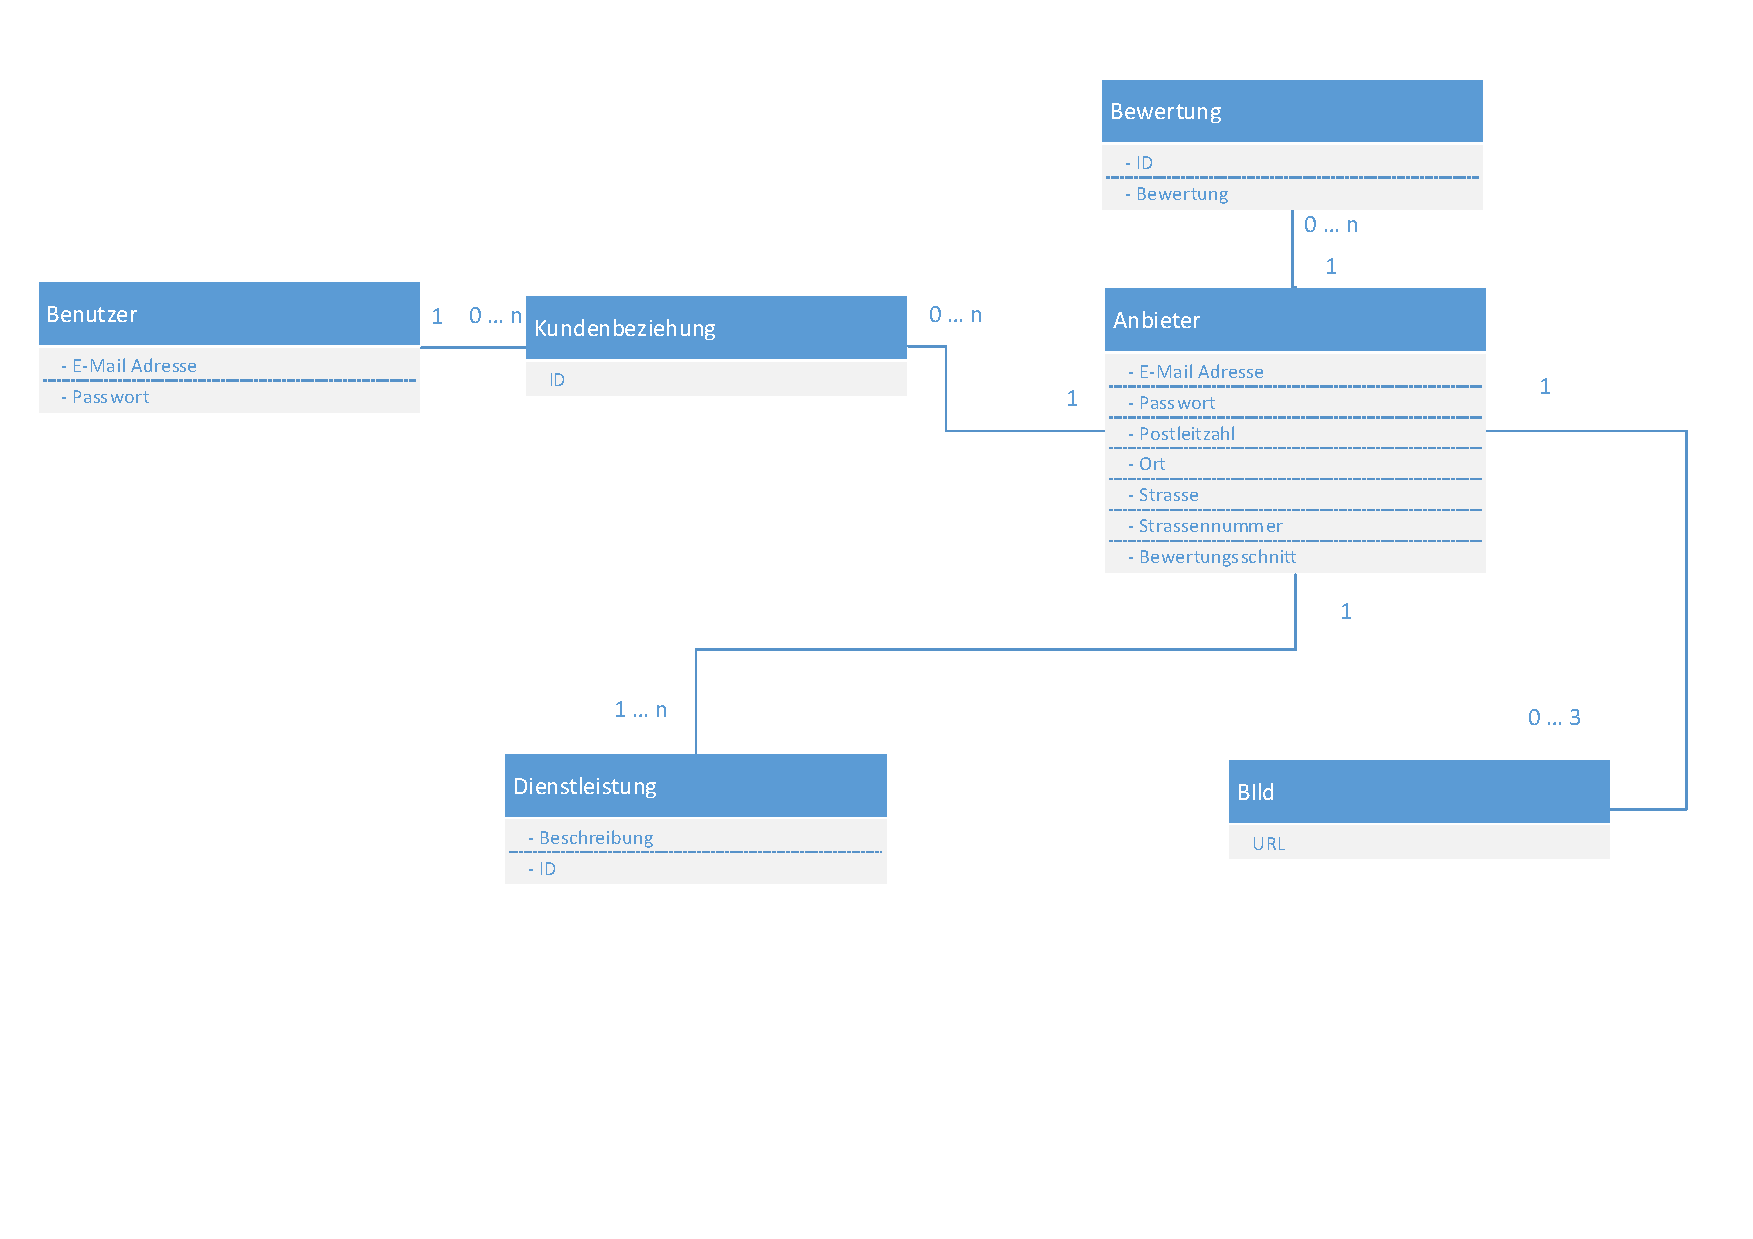
\includepdf[scale=0.7, pages=-, angle=90,pagecommand=\section{Datenmodell} \thispagestyle{headings}]{./Bilder/Datenmodell.pdf} 


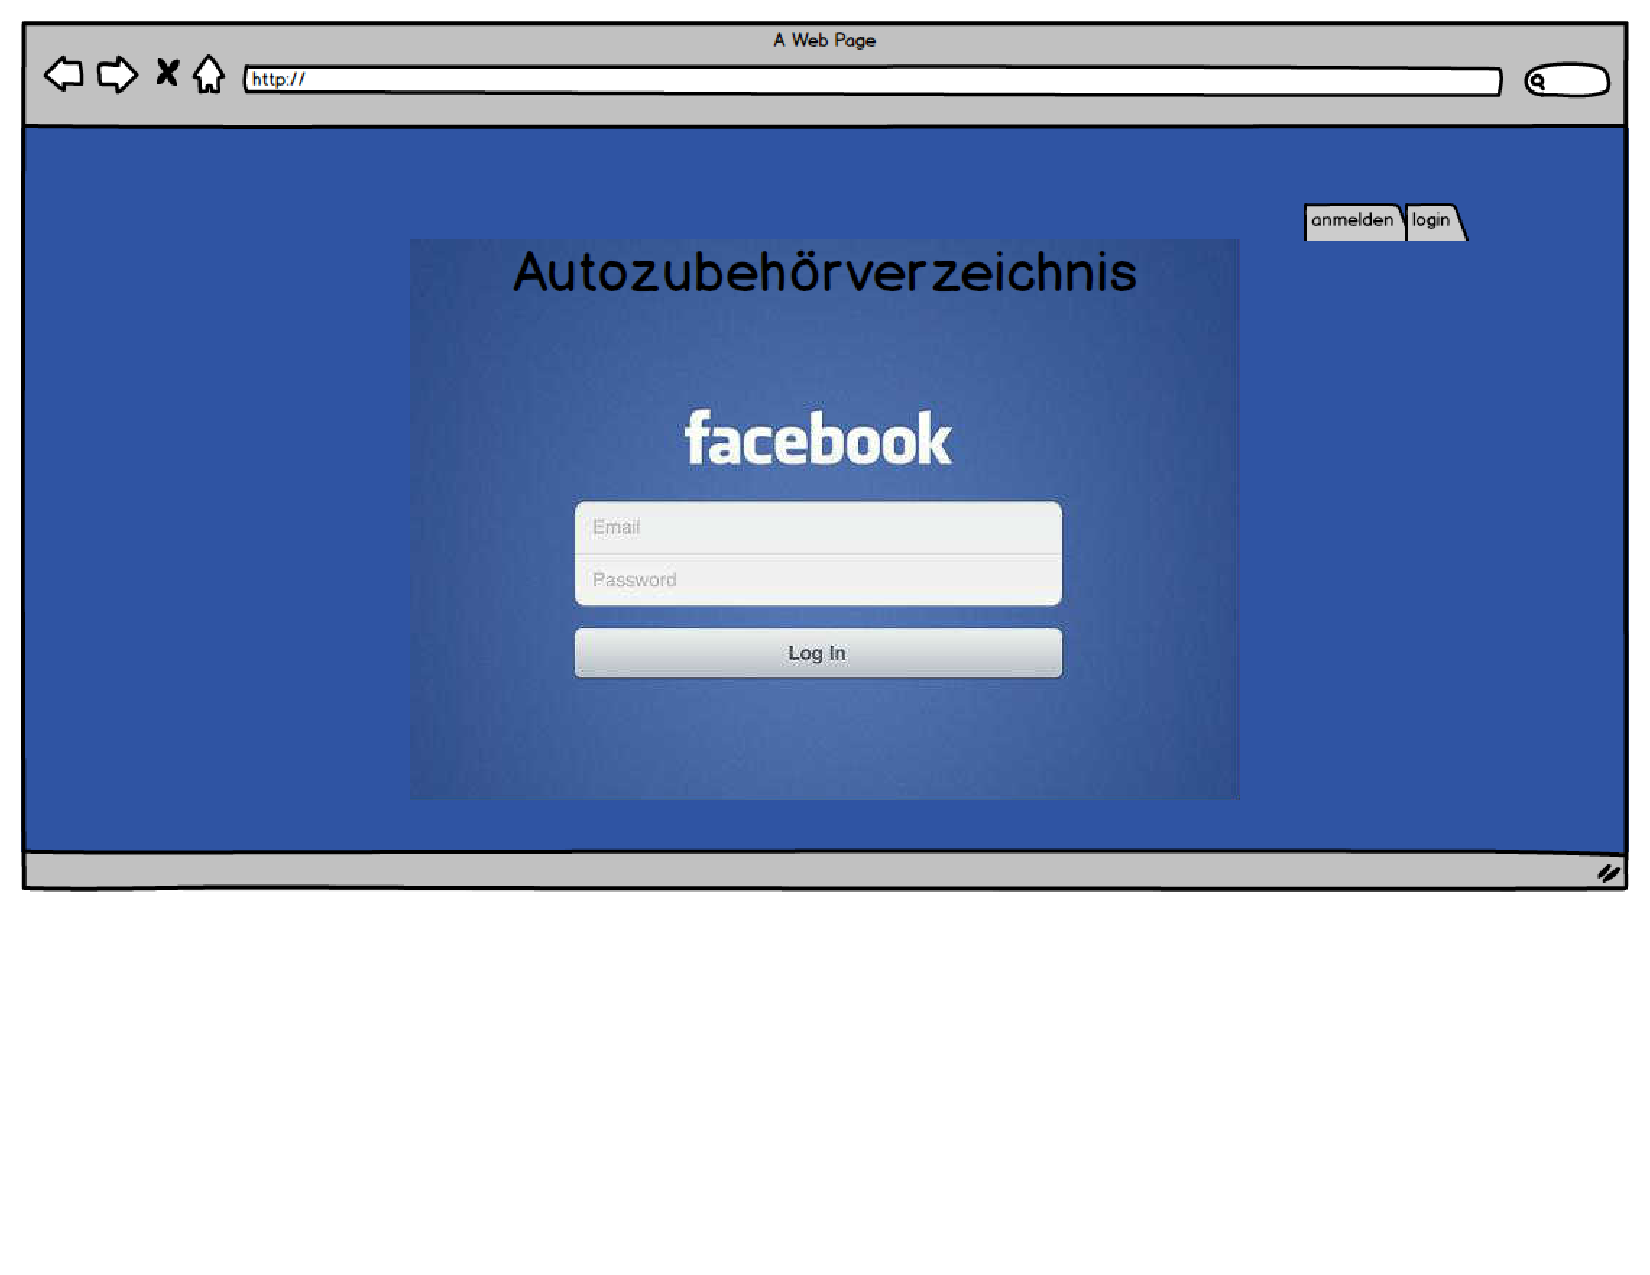
\includepdf[scale=0.75, pages=1-2, nup=1x2, angle=0,pagecommand=\section{Mockup} \thispagestyle{headings} ]{./Bilder/mockup.pdf} 
\includepdf[scale=0.75, pages=3-, nup=1x2, angle=0,pagecommand= \thispagestyle{headings} ]{./Bilder/mockup.pdf} 

\chapter{Architektur}
\section{Allgemein}
Die Webapplikation wurde mit dem Framework Bootstrap erstellt.
Um die Benutzung des JavaScript Codes zu vereinfachen, wurde die Bilbliotek JQuery verwendet. Für PHP wurde kein Framework verwendet.
Im folgenden ist der Facebook-Login und die Verwendung von Googlemaps in unserer Webapplikation beschrieben.\\

\noindent
\textbf{Links:}\\
GitHub-Repo: \url{https://github.com/tschoch/webapplikation}\\
Webapplikation: \url{http://614879-13.web.fh-htwchur.ch/projekt-web/Website/search_list.php}

\section{Facebook-Login}
Der Facebook login wurde mit dem PHP SDK \cite{phpsdk} von Facebook realisiert.
Um ein Facebook Login auf der eigenenen Seite zu ermöglichen, muss der Entwickler ein Facebook Developer Account \cite{fbdeveloper} erstellen. Danach kann die App auf der Facebook Developerseite erstellt werden und es wird eine App-ID und ein App-Secret generiert. Diese beiden credentials müssen in der Anfrage auf den Facebookserver mitgegeben werden, sonst funktioniert die Anfrage nicht.
Das Hauptskript für den Facebooklogin ist im folgenden beschrieben.\\

\begin{lstlisting}[language=PHP, frame=single, captionpos=b,caption= fbconfig.php]
<?php
// einbinden des Autoloaders
require_once 'autoload.php';

...
// Eingabe der App ID & des App Secret
FacebookSession::setDefaultApplication( 'App_ID','App_Secret' );

// erzeugen einer FacebookRedirectLoginHelper Instanz
$helper = new FacebookRedirectLoginHelper(
           'http://localhost/projekt_web/phplogin/fbconfig.php' );
try {

  //behandelt Facebook Rückmeldung und gibt Facebook Session zurück
  $session = $helper->getSessionFromRedirect();
} catch( FacebookRequestException $ex ) {
  // Wenn Facebook einen Error zurück gibt
} catch( Exception $ex ) {
  // Wenn die Überprüfung fehlschlägt oder andere Probleme
}

// Überprüfen ob Session vorhanden
if ( isset( $session ) ) {



  // graph api anfrage für user data
  $request = new FacebookRequest( 
  $request = new FacebookRequest( 
              $session, 'GET', '/me?locale=en_US&fields=id,name,email');
  $response = $request->execute();
  
  // Antwort mit Daten
  $graphObject = $response->getGraphObject();
        $fbid  = $graphObject->getProperty('id');
        $fbfullname = $graphObject->getProperty('name');
        $femail = $graphObject->getProperty('email');    

	    
   // Variablen in Session variablen abspeichern
   $_SESSION['FBID'] = $fbid;           
   $_SESSION['FULLNAME'] = $fbfullname;
   $_SESSION['EMAIL'] =  $femail;
    
   // DB aktualisieren
   checkuser($fbid,$fbfullname,$femail);
    
   //header location after session
   header("Location: ../Website/search_list.php");

// wenn noch keine Session   
} else {

  //Umleitung zur Loginseite, definition der genutzten daten
  $loginUrl = $helper->getLoginUrl( array('scope' => 'email'));
  header("Location: ".$loginUrl);
}
?>




 	    
\end{lstlisting}

\newpage
\noindent
Am Anfang einer Seite wird geprüft ob man bereits bei Facebook eingeloggt ist. Dies geschieht indem geprüft wird ob die Session variable FBID bereits gesetzt ist.

\begin{lstlisting}[language=PHP, frame=single, captionpos=b,caption= search\_list.php]
<?php
//session start
session_start(); 
...
//prüfe ob eingeloggt
if (\$_SESSION['FBID']):
...
php else: 
...
php endif 
?> 
\end{lstlisting}

\section{Maps}
\begin{lstlisting}[language=HTML, frame=single, captionpos=b]
<!DOCTYPE html>
<html>
<head>
    <style type="text/css">
      html, body { height: 100%; margin: 0; padding: 0; }
      #map { height: 100%; }
    </style>
  </head>
  <body>
    <div id="map"></div>
    <script type="text/javascript">
var map;
function initMap() {
  map = new google.maps.Map(document.getElementById('map'), {
    center: {lat: -34.397, lng: 150.644},
    zoom: 8
  });
}
    </script>
    <script async defer
      src="https://maps.googleapis.com/maps/api/js?
key=YOUR_API_KEY&callback=initMap">
    </script>
  </body>
</html>
\end{lstlisting}

\newpage
\noindent
Für die Suche auf der Karte wird Google Map verwendet, auf dem vorhergehendem Bild ist die Erstellung einer einfachen Karte zu sehen. Wichtig ist, damit man dies tun kann, einen Entwickler Account \cite{googledeveloper} bei Google zu machen , damit kann man sich dann einen API-Key für seine App generieren lassen.\\

\noindent
Um die Adressen aus der Datenbank auf der Map darzustellen muss aus der Adresse die Längen- und Breitengrade herausgefunden werden. Erneut liefert Google dazu ein API, genannt Geocode, welches einem dies abnimmt. Dabei wird die Adresse von welcher die Geolocation gesucht wird dem Parameter adress in der Adresszeile des \\ 
Browsers mitgegeben: \url{ https://maps.googleapis.com/maps/api/geocode/json?address=Pulverm
%C3%BChlestrasse+57,+7000+Chur }\cite{googlegeocode}
Die Antwort kommt in diesem Fall mit JSON zurück, alternativ wäre noch XML verfügbar. Um diese Antwort in JavaScript zu verarbeiten wird        

\begin{lstlisting}[ frame=single, captionpos=b,caption= script.php]
$.getJSON('http://maps.googleapis.com/maps/api/geocode/json? + 
address='+addresse+'&sensor=false', null, function (data) {
            var p = data.results[0].geometry.location
            var latlng = new google.maps.LatLng(p.lat, p.lng);
            new google.maps.Marker({
                position: latlng,
                map: map
            });
    });
\end{lstlisting}
aufgerufen. Mit dieser Funktion wird dynamisch ein Marker in der Map gesetzt. 

\newpage
\chapter{Test}
\textbf{Beschreibung}\\
Das Testen erfolgte vollkommen manuell, das heisst wir haben alle Tests selbst ausgeführt und nicht automatisiert. 
\begin{table}[H]
\begin{tabular}{|p{1.2cm}|p{1.2cm}| p{1.2cm}|p{1.2cm}|p{1.2cm}|p{1.2cm}|p{1.2cm}|p{1.2cm}|p{1.2cm}|p{1.2cm}|}\hline
      & T1 & T2 & T3 & T4 &T5 & T6 & T7 & T8 & T9 \\ \hline
  A.1 &  X &    &    &    &   &    &    &    &     \\ \hline
  A.2 &    &  X &    &    &   &    &    &    &     \\ \hline
  A.3 &    &  X &    &    &   &    &    &    &     \\ \hline
  A.4 &    &    &  X &    &   &    &    &    &     \\ \hline
  A.5 &    &    &    & X  & X &    &    &    &     \\ \hline
  A.6 &    &    &    &    &   & X  &    &    &     \\ \hline
  A.7 &    &    &    &    &   &    & X  &    &     \\ \hline
  A.8 &    &    &    &    &   &    &    &  X &     \\ \hline
  A.9 &    &    &    &    &   &    &    &    &  X  \\ \hline
 \end{tabular}
\caption{Traceability Matrix}
\end{table}
\section{Test 1}
10 Personen loggen sich mit Ihrem Facebook Profil auf der Seite ein. Anschliessend wird in der Datenbank überprüft ob Name, E-Mail Adresse und Facebook ID übergeben wurden. Alle 10 Benutzer wurden in der Datenbank übernommen mit den angeforderten Credentials. 
\newline
\begin{figure}[H]
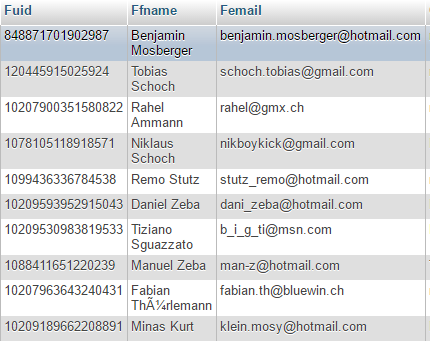
\includegraphics[height=9cm]{./Bilder/database.png}
\centering
\caption{Datenbankauszug Facebookdaten}
\end{figure}
\newpage


\section{Test 2}
Die Anwender(Dienstleister \& Benutzer) werden aufgefordert Ihr Profil im entsprechenden Edit-Fenster anzupassen, diese Änderung soll in der Datenbank ersichtlich sein. Alle 10 Benutzer haben Ihr Profil Ihren Wünschen nach angepasst und alle Werte wurden in der Datebank übernommen.
\newline
\begin{figure}[H]
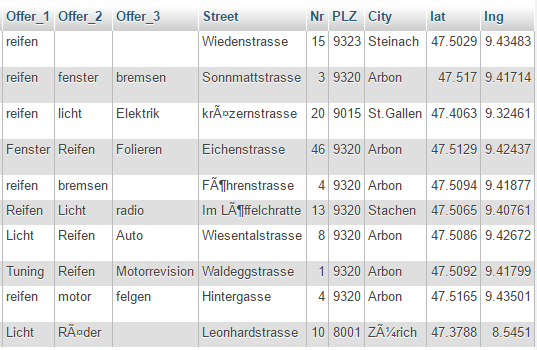
\includegraphics[height=10cm]{./Bilder/edit.png}
\centering
\caption{Datenbankauszug edit}
\end{figure}
\newpage


\section{Test 3}

5 Anfragen an die Webapplikation werden nur mit dem Suchbegriff ''Dienstleistung''  gestartet. Alle Dienstleister werden ausgegeben, bei welchem eine Dienstleistung dem Suchbegriff entspricht. 
\begin{table}[H]
\begin{tabular}{|p{2.4cm}|p{0.9cm}| p{0.9cm}|p{1.0cm}|p{1.1cm}|p{0.9cm}|p{1.2cm}|p{1.2cm}|p{1.5cm}|p{1.1cm}|p{1.1cm}|}\hline      			& Minas 	&  Rahel & Daniel   & Manuel 	&  Remo  & Tiziano   & Tobias   & Benjamin   &  Niklaus  &  Fabian    \\ \hline
  Reifen 	  	&    &  X &  X	& X  & X  & X  & X  & X  & X  & X    \\ \hline
  Radio 		&    &    &  X	&    &    &    &    &    &    &      \\ \hline
  Felgen		&    &    &   	&    &    &    &    &    &    & X    \\ \hline
  Motorrevision &    &    &   	& X  &    &    &    &    &    &      \\ \hline
  Fenster 		&    &    &   	&    &    &    & X  &    & X  &      \\ \hline
 \end{tabular}       
\caption{Test Dienstleistung}       
\end{table}      

\section{Test 4}

5 Anfragen an die Webapplikation werden nur mit dem Suchbegriff ''Ort'' gestartet. 
Es werden alle Dienstleister ausgegeben, bei welchen sich der Dienstleister in einem Umkreis von 5 km um den Ortskern befinden. Dies erklärt das gleiche Ergebnis bei Arbon und Steinach.

\begin{table}[H]
\begin{tabular}{|p{2.4cm}|p{0.9cm}| p{0.9cm}|p{1.0cm}|p{1.1cm}|p{0.9cm}|p{1.2cm}|p{1.2cm}|p{1.5cm}|p{1.1cm}|p{1.1cm}|}\hline      			& Minas 	&  Rahel & Daniel   & Manuel 	&  Remo  & Tiziano   & Tobias   & Benjamin   &  Niklaus  &  Fabian    \\ \hline
  Arbon 	  	&     &     &  X  &  X  &  X  &  X  &  X  &  X  &  X  &  X    \\ \hline
  Zürich 		&  X  &     &     &     &     &     &     &     &     &       \\ \hline
  St.Gallen		&     &  X  &     &     &     &     &     &     &     &       \\ \hline
  Chur 			&     &     &     &     &     &     &     &     &     &       \\ \hline
  Steinach 		&     &     &  X  &  X  &  X  &  X  &  X  &  X  &  X  &  X    \\ \hline
 \end{tabular}       
\caption{Test Ort} 
\end{table}      
\section{Test 5}

5 Anfragen an die Webapplikation werden nur mit dem Suchbegriff ''Radius'' gestartet. 
Es werden alle Dienstleister ausgegeben, bei welchen sich der Dienstleister in einem Umkreis um das geografische Zentrum der Schweiz befindet.

\begin{table}[H]
\begin{tabular}{|p{2.4cm}|p{0.9cm}| p{0.9cm}|p{1.0cm}|p{1.1cm}|p{0.9cm}|p{1.2cm}|p{1.2cm}|p{1.5cm}|p{1.1cm}|p{1.1cm}|}\hline      			& Minas 	&  Rahel & Daniel   & Manuel 	&  Remo  & Tiziano   & Tobias   & Benjamin   &  Niklaus  &  Fabian    \\ \hline
  50 km	  		&     &     &     &     &     &     &     &     &     &       \\ \hline
  75 km			&  X  &     &     &     &     &     &     &     &     &       \\ \hline
  110 km		&  X  &  X  &     &     &     &     &     &     &     &       \\ \hline
  113 km		&  X  &  X  &  X  &     &     &     &     &     &     &       \\ \hline
  125 km		&  X  &  X  &  X  &  X  &  X  &  X  &  X  &  X  &  X  &  X    \\ \hline
 \end{tabular}       
\caption{Test Radius}       
\end{table}      
\newpage
\section{Test 6}
5 Dienstleister werden nach einer ihrer Dienstleistungen mit unterschiedlichen Anzahl Sternen bewertet.
\begin{figure}[H]
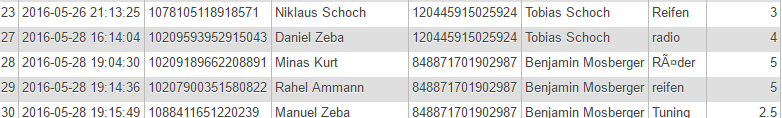
\includegraphics[height=2.5cm]{./Bilder/bewertung.png}
\centering
\caption{Datenbankauszug Bewertung}
\end{figure}

\section{Test 7}
Das Umschalten zwischen Map und Liste ist implementiert und es kann dazwischen umgeschaltet werden.
\section{Test 8}
\begin{figure}[H]
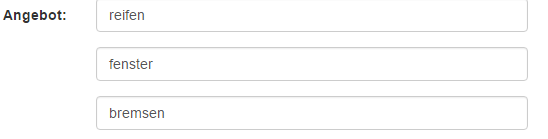
\includegraphics[height=4cm]{./Bilder/dienstleistung.png}
\centering
\caption{Edit-Ansicht Angebot}
\end{figure}
\section{Test 9}
\begin{figure}[H]
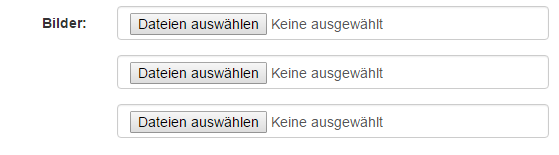
\includegraphics[height=4cm]{./Bilder/bilder.png}
\centering
\caption{Edit-Ansicht Bildupload}
\end{figure}

\newpage
%%\chapter{Vorgehen}


\chapter{Lessons-learned}
Wir haben uns von Anfang an gegen ein Framework entschieden, 
da wir uns diese Einarbeitungszeit sparen wollten, um dafür mehr Funktionalität einzubauen. Dies ist unserer Meinung nach gut gelungen und wir haben viel gelerntes repetieren können und unser Wissen auch in diese Richtungen erweitern können welche uns persönlich interessieren. Je grösser das Projekt wurde, desto mehr haben wir uns aber gewünscht wir hätten doch ein Framework verwendet, da viel Code doppelt vorgekommen ist und das auslagern der Übersichtlichkeit massiv geschadet hat. 

%%\chapter{Team-Dynamik}


\newpage
\begin{thebibliography}{999}

\bibitem{phpsdk}  Github. facebook-php-sdk-v4
 URL: \url{https://github.com/facebook/facebook-php-sdk-v4/} [Stand 6.4.2016].
 \bibitem{fbdeveloper}  Facebook Developer
 URL: \url{facebook developer conference} [Stand 31.5.2016].
 \bibitem{googledeveloper}  Google Developer
 URL: \url{https://developers.google.com} [Stand 31.5.2016].
  \bibitem{googlegeocode}  Google Geocode
 URL: \url{https://developers.google.com/maps/documentation/geocoding/intro?hl=de} [Stand 31.5.2016].
\end{thebibliography}
\end{document}









